\newpage
\section{Setting up your workspace}
\genHeader

To start any TGG Transformation, you need to have the source and target graphs already prepared. Our example will use the \texttt{LeitnersLearningBox}
metamodel (as completed in Parts II and III) as the transformation's source, and a new \texttt{DictionaryLanguage} as its target. We have provided this
second metamodel as a download.

If you haven't worked through the previous parts of this handbook, complete Section~\ref{sec:loadSourceMeta} first to load a pre-prepared learning box into your
workspace. If your source metamodel is ready however, skip ahead to either \texttt{\hyperlink{sec:multiEAP}{Section 2.2 (Visual)}} or
\texttt{\hyperlink{sec:multiMOSL}{Section 2.3 (Textual)}} to begin.


\subsection{Get Eclipse}
\label{sec:get-eclipse}

Navigate to \url{https://www.eclipse.org/downloads/} and download the latest \texttt{Eclipse Modeling Tools}.\footnote{We have tested this part of the handbook for \texttt{Eclipse Neon (4.6.0)} running on Windows 8.1.}
Do not try to use another Eclipse package as it probably won't work.

\subsection{Install eMoflon}
\label{sec:get-emoflon}

Install eMoflon as an Eclipse plugin from this update site.\footnote{\url{http://www.emoflon.org/fileadmin/download/moflon-ide/eclipse-plugin/beta/update-site2/}}
When installing, make sure you choose to install \emph{all} available features.

If you don't already have Graphviz dot installed on your system then install it:
\url{http://www.graphviz.org/Download.php}.
Make sure that the program \emph{dot} is accessible by adding the \emph{bin} directory of your Graphviz installation to the environment variable \%PATH\% (on Windows) or \$PATH (on Linux).

\subsection{Install your initial workspace}
\label{sec:loadSourceMeta}

To get started in Eclipse, press the \menuPath{Install, configure and deploy Moflon} button (\eMoflonMenuButton) and navigate to \menuPath{Install Workspace}.
Choose \menuPath{eMoflon Examples \menuSep Handbook Part 4 Start} (\Cref{eclipse:downPartIV}).
It contains the \texttt{Leitners\-Learning\-Box} and \texttt{Dictionary\-Language} metamodels, which we'll be using. 
By the way, don't freak out if your workspace looks slightly different than our screenshots -- things often change faster than we can update this handbook.
If the difference is important and confusing, however, please send us an email:  \emoflonMail.

If everything went well, you should now have two projects in your workspace.  
Go ahead and explore the metamodels (\texttt{/model/*.ecore}, \texttt{/model/*.aird}).
The generated code (\texttt{/gen}) is standard EMF code.

\begin{figure}[htbp]
\begin{center}
  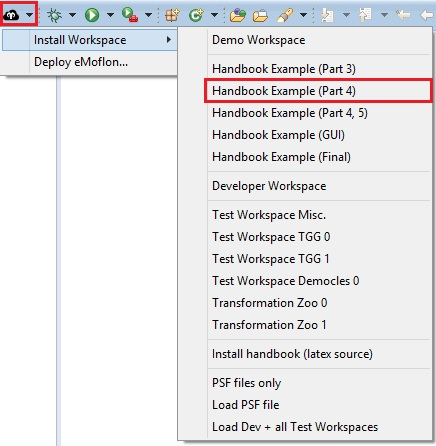
\includegraphics[width=0.65\textwidth]{eclipse_part4FreshWizardDownload}
  \caption{Initialize your workspace}
  \label{eclipse:downPartIV}
\end{center}
\end{figure} 

If you ever want to create your own meta-model, eMoflon provides a wizard (\menuPath{Create new repository project} (\eMoflonCreateNewRepositoryProjectIcon) in the eMoflon toolbar) for this, which creates the expected project structure with an empty ecore file that you can fill out.

%%% Local Variables: 
%%% mode: latex
%%% TeX-master: "../../src/TGG_mainFile"
%%% End: 


\jumpDual{multiEAP}{multiMOSL}

\newpage
\hypertarget{multiEAP}{}
\subsection{Importing and working with multiple EAPs}
\visHeader

Please note that the following instructions on how to properly export and import Enterprise Architect (EA) files are \emph{not} an eMoflon-exclusive feature.
We have included them here as part of our handbook as getting this right is crucial for working with eMoflon, especially when working with TGGs. The main
problem is that, as far as we know, EA does not (yet) support referencing model elements in one EAP from another, completely different EAP. This means that all
required metamodels have to first be merged in the same EAP before such references can be specified (as required for TGGs).

\begin{itemize}

\item[$\blacktriangleright$] Press the \texttt{new} button in the Eclipse toolbar and navigate to ``Examples/eMoflon Handbook Examples/''
(Fig.~\ref{eclipse:dictionaryDownloadWizard}). Find and select \texttt{Part IV Visual Dictionary Language} to copy a new \texttt{Dict\-ion\-ary\-Lang\-uage}
metamodel project into your workspace.

\vspace{0.5cm}

% Image stored in ../1_gettingStarted/textImportImages/  (repeated image)
\begin{figure}[htbp]
\begin{center}
  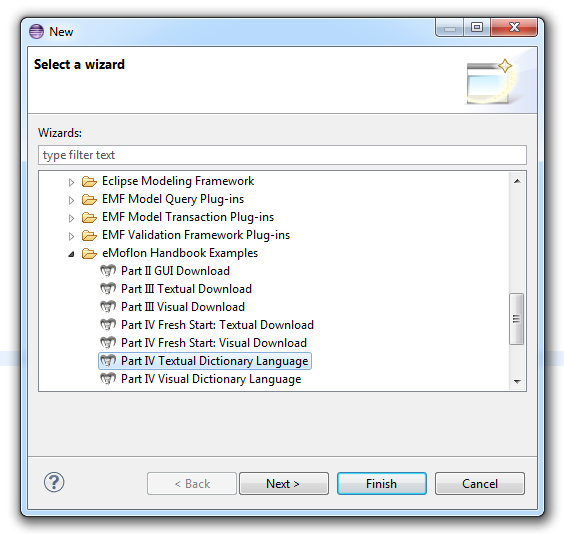
\includegraphics[width=0.8\textwidth]{eclipse_part4DictionaryLanguageDownload}
  \caption{Get the visual \texttt{DictionaryLanguage} metamodel}
  \label{eclipse:dictionaryDownloadWizard}
\end{center}
\end{figure}

\item[$\blacktriangleright$] If successful, your workspace should resemble Fig.~\ref{eclipse:loadedDictionaryEAP}. Double-click
\texttt{Dictionary.eap} to open it in EA.

\newpage

\begin{figure}[htbp]
\begin{center}
  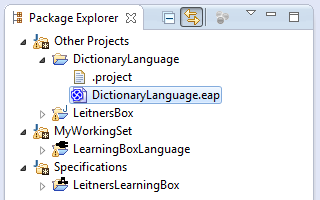
\includegraphics[width=0.5\textwidth]{eclipse_loadedDictionaryEAP}
  \caption{\texttt{Dictionary} metamodel successfully copied into the workspace}
  \label{eclipse:loadedDictionaryEAP}
\end{center}
\end{figure}

\item[$\blacktriangleright$] The file's project browser should resemble Fig.~\ref{ea:dictionaryLangStart}. Feel free to inspect the main
\texttt{DictionaryLanguage} diagram until you're familiar with the metamodel. Our work will be focused on the \texttt{Dictionary} and \texttt{Entry} classes.
You'll be able to see that dictionaries can be assigned unique \texttt{EString title}s, and each entry will have some sort of \texttt{content} matched with one
of three difficulty \texttt{level}s.

\vspace{0.5cm}

\begin{figure}[htbp]
\begin{center}
  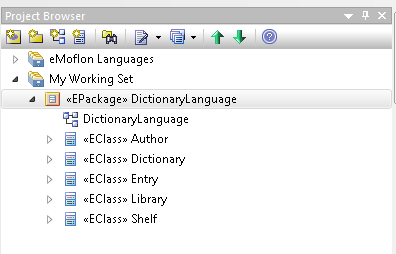
\includegraphics[width=0.4\textwidth]{ea_dictLangProBrowser}
  \caption{The \texttt{DictionaryLanguage} metamodel structure}
  \label{ea:dictionaryLangStart}
\end{center}
\end{figure}

\item[$\blacktriangleright$] It should be said that while you are able to simply copy and paste packages between multiple EAPs (i.e., copy
\texttt{<<E\-Pack\-age>>Dict\-ion\-ary\-Lang\-uage} into the \texttt{MyWorkingSet} root note of your source metamodel), if any of the copied packages have
dependencies on other packages, it cannot be done so easily. All links would be destroyed! 

\clearpage

\item[$\blacktriangleright$] Therefore, to properly migrate the \texttt{DictionaryLanguage} package, right-click on the EPackage root, navigate to
``Import/Export" and select \texttt{Export Model to XMI\ldots} (Fig.~\ref{ea:contextExport}). Alternatively, you can select the root in the project browser and
press \texttt{Ctrl + Alt + E}.

\vspace{0.5cm}

\begin{figure}[htbp]
\begin{center}
  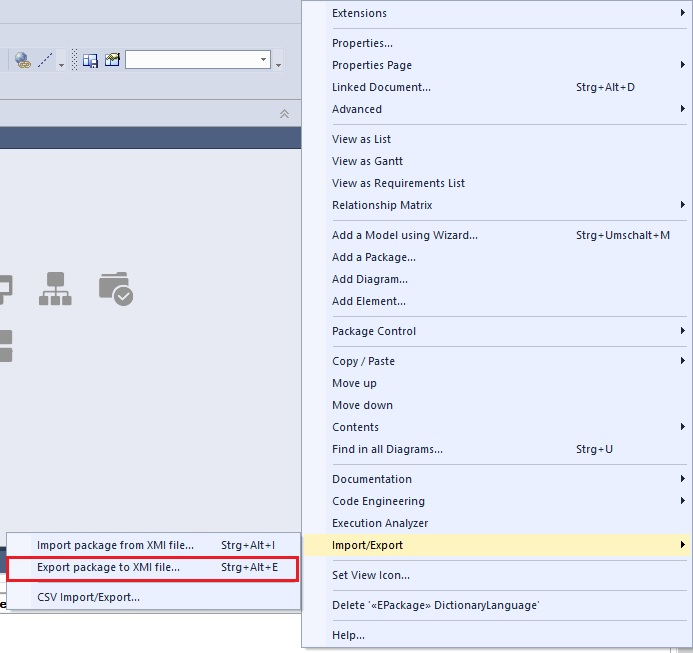
\includegraphics[width=\textwidth]{ea_contextExport}
  \caption{Starting the export process in EA}
  \label{ea:contextExport}
\end{center}
\end{figure}

\item[$\blacktriangleright$] Switch the export type to \texttt{XMI 2.1} in the dialogue and save the file somewhere easily accessible. Press export, and close
the window once the small green bar appears (Fig.~\ref{ea:export}).

\begin{figure}[htbp]
\begin{center}
  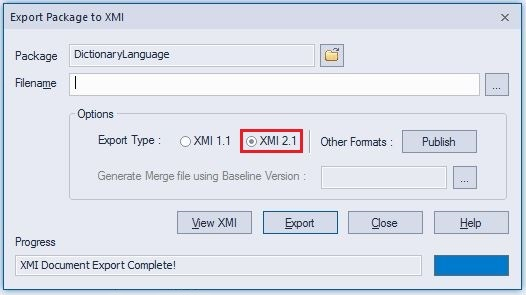
\includegraphics[width=0.9\textwidth]{ea_dialogueExport}
  \caption{Exporting the metamodel to a file}
  \label{ea:export}
\end{center}
\end{figure}

\item[$\blacktriangleright$] Go back to Eclipse and open \texttt{LeitnersLearningBox.eap}. Right-click on \texttt{MyWorkingSet} and navigate to ``Import
Model from XMI\ldots''

\item[$\blacktriangleright$] Find the \texttt{.xmi} file you just saved and press \texttt{import}. Press \texttt{OK} in the confirmation dialogue; Your project
browser should now resemble Fig.~\ref{ea:importProBrowser}, with both metamodels in the same working set, in the same EAP.

\begin{figure}[htbp]
\begin{center}
  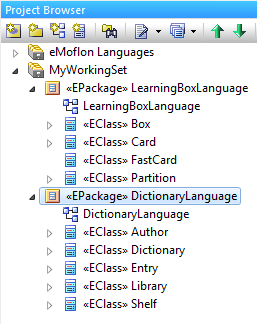
\includegraphics[width=0.5\textwidth]{ea_loadedDictionaryMetamodel}
  \caption{The TGG metamodels successfully included in one EAP}
  \label{ea:importProBrowser}
\end{center}
\end{figure}

\clearpage

\item[$\blacktriangleright$] Confirm the import by validating\footnote{To review the details of how to use the eMoflon control panel, read Section 2.8 from
Part II} (Fig.~\ref{ea:importValidationWindow}) and exporting the dual-metamodel project to Eclipse, refreshing \texttt{LeitnersLearningBox} to rebuild your workspace. 

\vspace{0.5cm}

\begin{figure}[htbp]
\begin{center}
  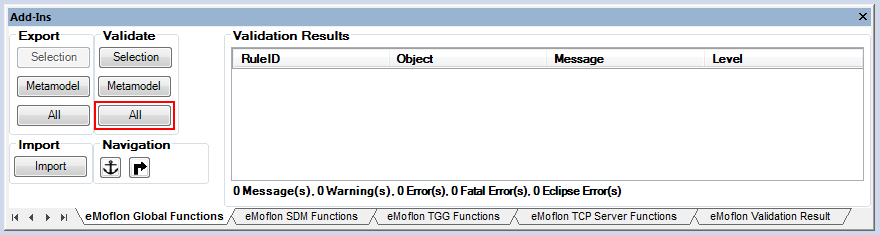
\includegraphics[width=\textwidth]{ea_importValidationWindow}
  \caption{No validation errors for \texttt{LeitnersLearningBox}}
  \label{ea:importValidationWindow}
\end{center}
\end{figure}

\vspace{0.5cm}

\item[$\blacktriangleright$] That's it! You now have the second metamodel for your transformation, and are ready to start specifying your TGG rules.

\jumpSingle{TGGSchema}

\end{itemize}


\newpage
\hypertarget{multiMOSL}{}
\subsection{Working with multple MOSL projects}
\texHeader

% Eclipse import instructions; all unconfirmed.
\begin{itemize}

\item[$\blacktriangleright$] Confirm your source metamodel \texttt{LeitnersLearningBox}, is in the current workspace prepared and right-click on
\texttt{MyWorkingSet}. Select \texttt{Import\ldots} from the context menu (Fig.~\ref{fig:eclipseContextImport}).

\vspace{0.25cm}

\begin{figure}[htbp]
\begin{center}
  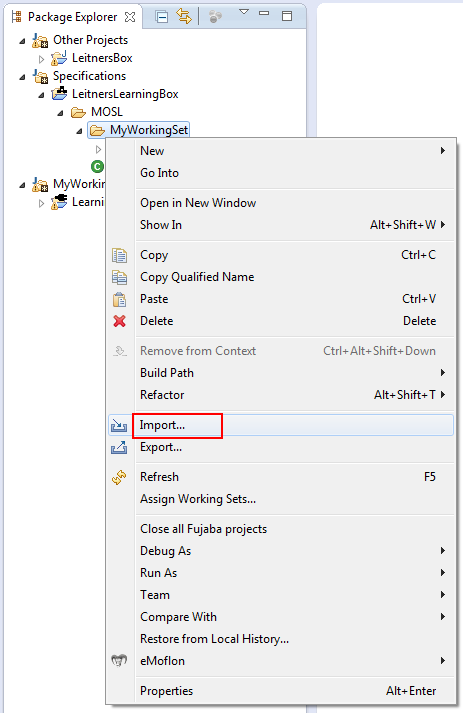
\includegraphics[width=0.6\textwidth]{eclipse_contextImport}
  \caption{caption}
  \label{fig:eclipseContextImport}
\end{center}
\end{figure}

\item[$\blacktriangleright$] In the first dialogue, set your import source by navigating to ``General/File System.'' This is the appropriate choice since
we want to import the entire directory structure of the target metamodel, not a pre existing project.

\item[$\blacktriangleright$] Press \texttt{Browse\ldots} and navigate to the folder where you extracted the contents of the \texttt{Part4.zip} download file
which included this document (Fig.~\ref{fig:importFileSys}). Press \texttt{Select All} to ensure you're importing all the necessary MOSL files for your TGG
target metamodel. Affirm and close the dialogue by pressing \texttt{Finish}.

\newpage

\begin{figure}[htbp]
\begin{center}
  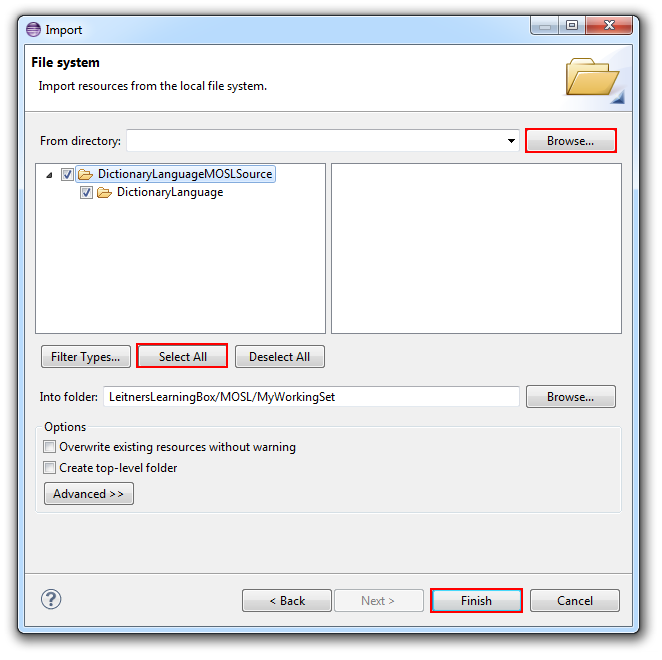
\includegraphics[width=0.8\textwidth]{eclipse_importDialogue}
  \caption{caption}
  \label{fig:importFileSys}
\end{center}
\end{figure}

\item[$\blacktriangleright$] With your project now loaded, navigate to ``Build (Without Cleaning)'' on the toolbar to build both metamodels. Confirm with
Fig.~\ref{fig:bothmetamodelstructures} that your MOSL directory is now populated with both metamodels, and notice that a second \texttt{Dictionary\-Language}
folder appeared under the same node as the \texttt{LearningBoxLanguage} repository project. If you expand this folder, you'll be able to see that it has
similar generated code for the imported metamodel.

\begin{figure}[htbp]
\begin{center}
  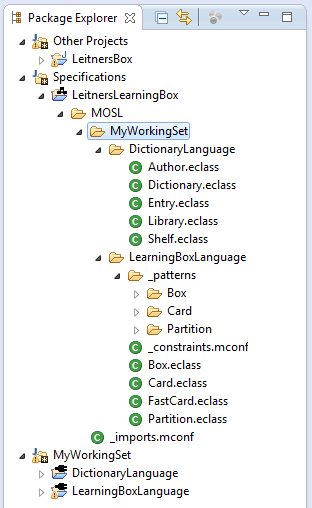
\includegraphics[width=0.5\textwidth]{eclipse_metamodelStructures}
  \caption{Fully loaded dual-metamodel structure}
  \label{fig:bothmetamodelstructures}
\end{center}
\end{figure}

\item[$\blacktriangleright$] Great work -- You're now ready to start using your metamodels in a TGG transformation! If you've just joined us and are interested
in the eMoflon project structure, or curious as to how Java code is generated, we invite you to read Section 4.2 from Part I. Otherwise, continue to the next section to begin
building your TGG Schema. 

\end{itemize}

